% Options for packages loaded elsewhere
\PassOptionsToPackage{unicode}{hyperref}
\PassOptionsToPackage{hyphens}{url}
\PassOptionsToPackage{dvipsnames,svgnames,x11names}{xcolor}
%
\documentclass[
  letterpaper,
  DIV=11,
  numbers=noendperiod]{scrartcl}

\usepackage{amsmath,amssymb}
\usepackage{iftex}
\ifPDFTeX
  \usepackage[T1]{fontenc}
  \usepackage[utf8]{inputenc}
  \usepackage{textcomp} % provide euro and other symbols
\else % if luatex or xetex
  \usepackage{unicode-math}
  \defaultfontfeatures{Scale=MatchLowercase}
  \defaultfontfeatures[\rmfamily]{Ligatures=TeX,Scale=1}
\fi
\usepackage{lmodern}
\ifPDFTeX\else  
    % xetex/luatex font selection
\fi
% Use upquote if available, for straight quotes in verbatim environments
\IfFileExists{upquote.sty}{\usepackage{upquote}}{}
\IfFileExists{microtype.sty}{% use microtype if available
  \usepackage[]{microtype}
  \UseMicrotypeSet[protrusion]{basicmath} % disable protrusion for tt fonts
}{}
\makeatletter
\@ifundefined{KOMAClassName}{% if non-KOMA class
  \IfFileExists{parskip.sty}{%
    \usepackage{parskip}
  }{% else
    \setlength{\parindent}{0pt}
    \setlength{\parskip}{6pt plus 2pt minus 1pt}}
}{% if KOMA class
  \KOMAoptions{parskip=half}}
\makeatother
\usepackage{xcolor}
\setlength{\emergencystretch}{3em} % prevent overfull lines
\setcounter{secnumdepth}{-\maxdimen} % remove section numbering
% Make \paragraph and \subparagraph free-standing
\makeatletter
\ifx\paragraph\undefined\else
  \let\oldparagraph\paragraph
  \renewcommand{\paragraph}{
    \@ifstar
      \xxxParagraphStar
      \xxxParagraphNoStar
  }
  \newcommand{\xxxParagraphStar}[1]{\oldparagraph*{#1}\mbox{}}
  \newcommand{\xxxParagraphNoStar}[1]{\oldparagraph{#1}\mbox{}}
\fi
\ifx\subparagraph\undefined\else
  \let\oldsubparagraph\subparagraph
  \renewcommand{\subparagraph}{
    \@ifstar
      \xxxSubParagraphStar
      \xxxSubParagraphNoStar
  }
  \newcommand{\xxxSubParagraphStar}[1]{\oldsubparagraph*{#1}\mbox{}}
  \newcommand{\xxxSubParagraphNoStar}[1]{\oldsubparagraph{#1}\mbox{}}
\fi
\makeatother

\usepackage{color}
\usepackage{fancyvrb}
\newcommand{\VerbBar}{|}
\newcommand{\VERB}{\Verb[commandchars=\\\{\}]}
\DefineVerbatimEnvironment{Highlighting}{Verbatim}{commandchars=\\\{\}}
% Add ',fontsize=\small' for more characters per line
\usepackage{framed}
\definecolor{shadecolor}{RGB}{241,243,245}
\newenvironment{Shaded}{\begin{snugshade}}{\end{snugshade}}
\newcommand{\AlertTok}[1]{\textcolor[rgb]{0.68,0.00,0.00}{#1}}
\newcommand{\AnnotationTok}[1]{\textcolor[rgb]{0.37,0.37,0.37}{#1}}
\newcommand{\AttributeTok}[1]{\textcolor[rgb]{0.40,0.45,0.13}{#1}}
\newcommand{\BaseNTok}[1]{\textcolor[rgb]{0.68,0.00,0.00}{#1}}
\newcommand{\BuiltInTok}[1]{\textcolor[rgb]{0.00,0.23,0.31}{#1}}
\newcommand{\CharTok}[1]{\textcolor[rgb]{0.13,0.47,0.30}{#1}}
\newcommand{\CommentTok}[1]{\textcolor[rgb]{0.37,0.37,0.37}{#1}}
\newcommand{\CommentVarTok}[1]{\textcolor[rgb]{0.37,0.37,0.37}{\textit{#1}}}
\newcommand{\ConstantTok}[1]{\textcolor[rgb]{0.56,0.35,0.01}{#1}}
\newcommand{\ControlFlowTok}[1]{\textcolor[rgb]{0.00,0.23,0.31}{\textbf{#1}}}
\newcommand{\DataTypeTok}[1]{\textcolor[rgb]{0.68,0.00,0.00}{#1}}
\newcommand{\DecValTok}[1]{\textcolor[rgb]{0.68,0.00,0.00}{#1}}
\newcommand{\DocumentationTok}[1]{\textcolor[rgb]{0.37,0.37,0.37}{\textit{#1}}}
\newcommand{\ErrorTok}[1]{\textcolor[rgb]{0.68,0.00,0.00}{#1}}
\newcommand{\ExtensionTok}[1]{\textcolor[rgb]{0.00,0.23,0.31}{#1}}
\newcommand{\FloatTok}[1]{\textcolor[rgb]{0.68,0.00,0.00}{#1}}
\newcommand{\FunctionTok}[1]{\textcolor[rgb]{0.28,0.35,0.67}{#1}}
\newcommand{\ImportTok}[1]{\textcolor[rgb]{0.00,0.46,0.62}{#1}}
\newcommand{\InformationTok}[1]{\textcolor[rgb]{0.37,0.37,0.37}{#1}}
\newcommand{\KeywordTok}[1]{\textcolor[rgb]{0.00,0.23,0.31}{\textbf{#1}}}
\newcommand{\NormalTok}[1]{\textcolor[rgb]{0.00,0.23,0.31}{#1}}
\newcommand{\OperatorTok}[1]{\textcolor[rgb]{0.37,0.37,0.37}{#1}}
\newcommand{\OtherTok}[1]{\textcolor[rgb]{0.00,0.23,0.31}{#1}}
\newcommand{\PreprocessorTok}[1]{\textcolor[rgb]{0.68,0.00,0.00}{#1}}
\newcommand{\RegionMarkerTok}[1]{\textcolor[rgb]{0.00,0.23,0.31}{#1}}
\newcommand{\SpecialCharTok}[1]{\textcolor[rgb]{0.37,0.37,0.37}{#1}}
\newcommand{\SpecialStringTok}[1]{\textcolor[rgb]{0.13,0.47,0.30}{#1}}
\newcommand{\StringTok}[1]{\textcolor[rgb]{0.13,0.47,0.30}{#1}}
\newcommand{\VariableTok}[1]{\textcolor[rgb]{0.07,0.07,0.07}{#1}}
\newcommand{\VerbatimStringTok}[1]{\textcolor[rgb]{0.13,0.47,0.30}{#1}}
\newcommand{\WarningTok}[1]{\textcolor[rgb]{0.37,0.37,0.37}{\textit{#1}}}

\providecommand{\tightlist}{%
  \setlength{\itemsep}{0pt}\setlength{\parskip}{0pt}}\usepackage{longtable,booktabs,array}
\usepackage{calc} % for calculating minipage widths
% Correct order of tables after \paragraph or \subparagraph
\usepackage{etoolbox}
\makeatletter
\patchcmd\longtable{\par}{\if@noskipsec\mbox{}\fi\par}{}{}
\makeatother
% Allow footnotes in longtable head/foot
\IfFileExists{footnotehyper.sty}{\usepackage{footnotehyper}}{\usepackage{footnote}}
\makesavenoteenv{longtable}
\usepackage{graphicx}
\makeatletter
\def\maxwidth{\ifdim\Gin@nat@width>\linewidth\linewidth\else\Gin@nat@width\fi}
\def\maxheight{\ifdim\Gin@nat@height>\textheight\textheight\else\Gin@nat@height\fi}
\makeatother
% Scale images if necessary, so that they will not overflow the page
% margins by default, and it is still possible to overwrite the defaults
% using explicit options in \includegraphics[width, height, ...]{}
\setkeys{Gin}{width=\maxwidth,height=\maxheight,keepaspectratio}
% Set default figure placement to htbp
\makeatletter
\def\fps@figure{htbp}
\makeatother

\KOMAoption{captions}{tableheading}
\makeatletter
\@ifpackageloaded{caption}{}{\usepackage{caption}}
\AtBeginDocument{%
\ifdefined\contentsname
  \renewcommand*\contentsname{Table of contents}
\else
  \newcommand\contentsname{Table of contents}
\fi
\ifdefined\listfigurename
  \renewcommand*\listfigurename{List of Figures}
\else
  \newcommand\listfigurename{List of Figures}
\fi
\ifdefined\listtablename
  \renewcommand*\listtablename{List of Tables}
\else
  \newcommand\listtablename{List of Tables}
\fi
\ifdefined\figurename
  \renewcommand*\figurename{Figure}
\else
  \newcommand\figurename{Figure}
\fi
\ifdefined\tablename
  \renewcommand*\tablename{Table}
\else
  \newcommand\tablename{Table}
\fi
}
\@ifpackageloaded{float}{}{\usepackage{float}}
\floatstyle{ruled}
\@ifundefined{c@chapter}{\newfloat{codelisting}{h}{lop}}{\newfloat{codelisting}{h}{lop}[chapter]}
\floatname{codelisting}{Listing}
\newcommand*\listoflistings{\listof{codelisting}{List of Listings}}
\makeatother
\makeatletter
\makeatother
\makeatletter
\@ifpackageloaded{caption}{}{\usepackage{caption}}
\@ifpackageloaded{subcaption}{}{\usepackage{subcaption}}
\makeatother

\ifLuaTeX
  \usepackage{selnolig}  % disable illegal ligatures
\fi
\usepackage{bookmark}

\IfFileExists{xurl.sty}{\usepackage{xurl}}{} % add URL line breaks if available
\urlstyle{same} % disable monospaced font for URLs
\hypersetup{
  pdftitle={Causal Directed Acylic Graphs},
  pdfauthor={Wouter van Amsterdam},
  colorlinks=true,
  linkcolor={blue},
  filecolor={Maroon},
  citecolor={Blue},
  urlcolor={Blue},
  pdfcreator={LaTeX via pandoc}}


\title{Causal Directed Acylic Graphs}
\usepackage{etoolbox}
\makeatletter
\providecommand{\subtitle}[1]{% add subtitle to \maketitle
  \apptocmd{\@title}{\par {\large #1 \par}}{}{}
}
\makeatother
\subtitle{introduction}
\author{Wouter van Amsterdam}
\date{2024-08-06}

\begin{document}
\maketitle

\renewcommand*\contentsname{Table of contents}
{
\hypersetup{linkcolor=}
\setcounter{tocdepth}{1}
\tableofcontents
}

\subsection{Causal inference
frameworks}\label{causal-inference-frameworks}

\subsubsection{What are they for?}\label{what-are-they-for}

\paragraph{Mathematical language to}\label{mathematical-language-to}

\begin{itemize}
\tightlist
\item
  define \emph{causal} quantities
\item
  express \emph{assumptions}
\item
  derive how to \emph{estimate} causal effects
\end{itemize}

\subsection{Causal inference
frameworks}\label{causal-inference-frameworks-1}

\subsubsection{Why learn more than one?}\label{why-learn-more-than-one}

\begin{itemize}
\tightlist
\item
  On day 1 we learned about the Potential Outcomes framework

  \begin{itemize}
  \tightlist
  \item
    Defines causal effects in terms of (averages of) \emph{individual
    potential outcomes}
  \item
    Estimation requires assumptions of (conditional) exchangeability and
    positivity / overlap and consistency
  \end{itemize}
\item
  There isn't only 1 way to think about causality, find one that
  `\emph{clicks}'
\item
  Now we will learn another framework: \emph{Structural Causal Models}
  and \emph{causal graphs}

  \begin{itemize}
  \tightlist
  \item
    causal relations and manipulations of \emph{variables}
  \item
    Developed by different people initially - Judea Pearl, Peter
    Spirtes, Clark Glymour
  \item
    SCM approach is broader in that it can define more different types
    of causal questions
  \end{itemize}
\item
  Equivalence: given the same data and assumptions, get the same
  estimates
\end{itemize}

\subsection{lecture 1 topics}\label{lecture-1-topics}

\begin{itemize}
\tightlist
\item
  why use DAGs
\item
\item
  what are DAGs and where do come from
\item
  SCMs as computer programs

  \begin{itemize}
  \tightlist
  \item
    intervention as change in program
  \end{itemize}
\item
  causal identifyability with DAGs

  \begin{itemize}
  \tightlist
  \item
    variable types: confounders, mediators, colliders (tinder: hot and
    intelligent / single ;on tinder)

    \begin{itemize}
    \tightlist
    \item
      confounders; storks; randomized, breaking arrows
    \end{itemize}
  \item
    d-separation
  \item
    back-door criterion
  \item
    follow rules of do calculus
  \end{itemize}
\item
  DAG
\end{itemize}

\begin{enumerate}
\def\labelenumi{\arabic{enumi}.}
\tightlist
\item
  what is the world
\item
  what can we estimate and how?
\item
  confounders / colliders
\item
  backdoor
\end{enumerate}

\subsection{lecture 2 topics}\label{lecture-2-topics}

\begin{itemize}
\tightlist
\item
  perfect versus soft intervention
\item
  critique of scm / cross-world assumptions
\end{itemize}

\subsection{practical 1}\label{practical-1}

\begin{itemize}
\tightlist
\item
  drawing and using dags (what to condition on); daggity
\item
  same data, different dags, different answers
\end{itemize}

\subsection{lecture 3 topics}\label{lecture-3-topics}

\begin{itemize}
\tightlist
\item
  bonus queries:

  \begin{itemize}
  \tightlist
  \item
    counterfactuals
  \item
    probability of necessity, probability of sufficiency
  \item
    actual causality (Joe Halpern)
  \end{itemize}
\item
  Pearl Causal Hierarchy
\item
  other uses of DAGs: missing data, selection
\item
  reflections on DAGs, limitations
\end{itemize}

\subsection{practical 2}\label{practical-2}

\begin{itemize}
\tightlist
\item
  causal ladder: what Q is this?
\item
  give data of hierarchy and answer the Q
\item
  give data of 2 treatments + SCM (treatment 3 which can be extrapolated
  from)
\end{itemize}

\section{Why are DAGs useful}\label{why-are-dags-useful}

\subsection{Example task: are hospital deliveries good for
babies?}\label{example-task-are-hospital-deliveries-good-for-babies}

\includegraphics{figs/delivery1.png}

\includegraphics{figs/delivery2.png}

\includegraphics{figs/delivery.png}

\subsection{Example task: are hospital deliveries good for
babies?}\label{example-task-are-hospital-deliveries-good-for-babies-1}

\begin{itemize}
\tightlist
\item
  You're a data scientist in the Wilhelmina Kinderziekenhuis (WKZ)
\item
  Have data on

  \begin{itemize}
  \tightlist
  \item
    delivery location (home or hospital)
  \item
    neonatal outcomes (good or bad)
  \item
    pregnancy risk (high or low)
  \end{itemize}
\item
  Question: do hospital deliveries result in better outcomes for babies?
\end{itemize}

. . .

\begin{Shaded}
\begin{Highlighting}[]
\CommentTok{\# t=0: home, t=1: hospital}
\CommentTok{\# z=0: low risk, z=1: high risk}
\CommentTok{\# y=1: good outcome}
\NormalTok{dnames }\OtherTok{=} \FunctionTok{list}\NormalTok{(}\AttributeTok{location=}\FunctionTok{c}\NormalTok{(}\StringTok{\textquotesingle{}home\textquotesingle{}}\NormalTok{, }\StringTok{\textquotesingle{}hospital\textquotesingle{}}\NormalTok{), }\AttributeTok{risk=}\FunctionTok{c}\NormalTok{(}\StringTok{\textquotesingle{}low\textquotesingle{}}\NormalTok{, }\StringTok{\textquotesingle{}high\textquotesingle{}}\NormalTok{))}
\NormalTok{pos\_tz }\OtherTok{\textless{}{-}} \FunctionTok{matrix}\NormalTok{(}\FunctionTok{c}\NormalTok{(}
  \FunctionTok{c}\NormalTok{(}\FloatTok{0.9}\NormalTok{,  }\FloatTok{0.5}\NormalTok{), }\CommentTok{\# y|t=0,z=0,1}
  \FunctionTok{c}\NormalTok{(}\FloatTok{0.95}\NormalTok{, }\FloatTok{0.8}\NormalTok{)  }\CommentTok{\# y|t=1,z=0,1}
\NormalTok{), }\AttributeTok{nrow=}\DecValTok{2}\NormalTok{, }\AttributeTok{byrow=}\NormalTok{T,}
\AttributeTok{dimnames=}\NormalTok{dnames)}

\NormalTok{ps\_tz }\OtherTok{\textless{}{-}} \FunctionTok{matrix}\NormalTok{(}\FunctionTok{c}\NormalTok{(}
  \FunctionTok{c}\NormalTok{(}\FloatTok{0.72}\NormalTok{, }\FloatTok{0.08}\NormalTok{), }\CommentTok{\# p(t=0,z=0,1)}
  \FunctionTok{c}\NormalTok{(}\FloatTok{0.02}\NormalTok{, }\FloatTok{0.18}\NormalTok{)  }\CommentTok{\# p(t=1,z=0,1)}
\NormalTok{), }\AttributeTok{nrow=}\DecValTok{2}\NormalTok{, }\AttributeTok{byrow=}\NormalTok{T, }\AttributeTok{dimnames=}\NormalTok{dnames)}

\CommentTok{\# p(t,z) under do(t)}
\NormalTok{ps\_do0 }\OtherTok{\textless{}{-}} \FunctionTok{matrix}\NormalTok{(}\FunctionTok{c}\NormalTok{( }
  \FunctionTok{c}\NormalTok{(}\FloatTok{0.8}\NormalTok{, }\FloatTok{0.2}\NormalTok{), }
  \FunctionTok{c}\NormalTok{(}\FloatTok{0.0}\NormalTok{, }\FloatTok{0.0}\NormalTok{)  }
\NormalTok{), }\AttributeTok{nrow=}\DecValTok{2}\NormalTok{, }\AttributeTok{byrow=}\NormalTok{T)}

\NormalTok{ps\_do1 }\OtherTok{\textless{}{-}} \FunctionTok{matrix}\NormalTok{(}\FunctionTok{c}\NormalTok{( }
  \FunctionTok{c}\NormalTok{(}\FloatTok{0.0}\NormalTok{, }\FloatTok{0.0}\NormalTok{), }
  \FunctionTok{c}\NormalTok{(}\FloatTok{0.8}\NormalTok{, }\FloatTok{0.2}\NormalTok{) }
\NormalTok{), }\AttributeTok{nrow=}\DecValTok{2}\NormalTok{, }\AttributeTok{byrow=}\NormalTok{T)}


\NormalTok{eys  }\OtherTok{\textless{}{-}} \FunctionTok{rowSums}\NormalTok{(pos\_tz }\SpecialCharTok{*}\NormalTok{ ps\_tz) }\SpecialCharTok{/} \FunctionTok{rowSums}\NormalTok{(ps\_tz) }\CommentTok{\# E y|t}
\NormalTok{dots }\OtherTok{\textless{}{-}} \FunctionTok{c}\NormalTok{(}\FunctionTok{sum}\NormalTok{(pos\_tz }\SpecialCharTok{*}\NormalTok{ ps\_do0), }\FunctionTok{sum}\NormalTok{(pos\_tz}\SpecialCharTok{*}\NormalTok{ps\_do1))}

\NormalTok{n }\OtherTok{=} \DecValTok{1000}

\NormalTok{ts  }\OtherTok{\textless{}{-}} \FunctionTok{vector}\NormalTok{(}\AttributeTok{mode=}\StringTok{"logical"}\NormalTok{, }\AttributeTok{length=}\DecValTok{0}\NormalTok{)}
\NormalTok{zs  }\OtherTok{\textless{}{-}} \FunctionTok{vector}\NormalTok{(}\AttributeTok{mode=}\StringTok{"logical"}\NormalTok{, }\AttributeTok{length=}\DecValTok{0}\NormalTok{)}
\NormalTok{py0s }\OtherTok{\textless{}{-}} \FunctionTok{vector}\NormalTok{(}\AttributeTok{mode=}\StringTok{"numeric"}\NormalTok{, }\AttributeTok{length=}\DecValTok{0}\NormalTok{)}
\NormalTok{py1s }\OtherTok{\textless{}{-}} \FunctionTok{vector}\NormalTok{(}\AttributeTok{mode=}\StringTok{"numeric"}\NormalTok{, }\AttributeTok{length=}\DecValTok{0}\NormalTok{)}
\NormalTok{ys  }\OtherTok{\textless{}{-}} \FunctionTok{vector}\NormalTok{(}\AttributeTok{mode=}\StringTok{"logical"}\NormalTok{, }\AttributeTok{length=}\DecValTok{0}\NormalTok{)}

\NormalTok{ntots }\OtherTok{\textless{}{-}}\NormalTok{ n }\SpecialCharTok{*}\NormalTok{ ps\_tz}

\ControlFlowTok{for}\NormalTok{ (t }\ControlFlowTok{in} \FunctionTok{c}\NormalTok{(}\DecValTok{0}\NormalTok{,}\DecValTok{1}\NormalTok{)) \{}
  \ControlFlowTok{for}\NormalTok{ (z }\ControlFlowTok{in} \FunctionTok{c}\NormalTok{(}\DecValTok{0}\NormalTok{,}\DecValTok{1}\NormalTok{)) \{}
\NormalTok{    ntz }\OtherTok{\textless{}{-}}\NormalTok{ n }\SpecialCharTok{*}\NormalTok{ps\_tz[t}\SpecialCharTok{+}\DecValTok{1}\NormalTok{,z}\SpecialCharTok{+}\DecValTok{1}\NormalTok{]}
\NormalTok{    ts  }\OtherTok{\textless{}{-}} \FunctionTok{c}\NormalTok{(ts, }\FunctionTok{rep}\NormalTok{(t, ntz))}
\NormalTok{    zs  }\OtherTok{\textless{}{-}} \FunctionTok{c}\NormalTok{(zs, }\FunctionTok{rep}\NormalTok{(z, ntz))}
\NormalTok{    py }\OtherTok{\textless{}{-}}\NormalTok{ pos\_tz[t}\SpecialCharTok{+}\DecValTok{1}\NormalTok{,z}\SpecialCharTok{+}\DecValTok{1}\NormalTok{]}
\NormalTok{    y }\OtherTok{\textless{}{-}} \FunctionTok{c}\NormalTok{(}\FunctionTok{rep}\NormalTok{(}\DecValTok{0}\NormalTok{,}
               \FunctionTok{round}\NormalTok{(ntz }\SpecialCharTok{*}\NormalTok{ (}\DecValTok{1}\SpecialCharTok{{-}}\NormalTok{py))), }\CommentTok{\# \textless{}{-} round should not be needed here but found a bug}
           \FunctionTok{rep}\NormalTok{(}\DecValTok{1}\NormalTok{,}
               \FunctionTok{round}\NormalTok{(ntz}\SpecialCharTok{*}\NormalTok{py))) }
\NormalTok{    ys }\OtherTok{\textless{}{-}} \FunctionTok{c}\NormalTok{(ys, y)}
\NormalTok{    py0s }\OtherTok{\textless{}{-}} \FunctionTok{c}\NormalTok{(py0s, }\FunctionTok{rep}\NormalTok{(pos\_tz[}\DecValTok{1}\NormalTok{, z}\SpecialCharTok{+}\DecValTok{1}\NormalTok{], ntz))}
\NormalTok{    py1s }\OtherTok{\textless{}{-}} \FunctionTok{c}\NormalTok{(py1s, }\FunctionTok{rep}\NormalTok{(pos\_tz[}\DecValTok{2}\NormalTok{, z}\SpecialCharTok{+}\DecValTok{1}\NormalTok{], ntz))}
\NormalTok{  \}}
\NormalTok{\}}
\CommentTok{\# ys \textless{}{-} ifelse(ts, y1s, y0s)}
\NormalTok{df }\OtherTok{\textless{}{-}} \FunctionTok{data.table}\NormalTok{(}
  \AttributeTok{location=}\NormalTok{ts,}
  \AttributeTok{risk=}\NormalTok{zs,}
  \AttributeTok{outcome=}\NormalTok{ys,}
  \AttributeTok{py0=}\NormalTok{py0s,}
  \AttributeTok{py1=}\NormalTok{py1s)}

\CommentTok{\# head(df)}

\CommentTok{\# kable(eys, col.names="tips")}
\CommentTok{\#pander::pander(ftable(eys))}

\CommentTok{\# pander::pander(ftable(pos\_tz), emphasize.strong.rows=c(1), emphasize.strong.cols=c(1))}

\NormalTok{ntots }\OtherTok{\textless{}{-}}\NormalTok{ n }\SpecialCharTok{*}\NormalTok{ ps\_tz}
\NormalTok{nys }\OtherTok{\textless{}{-}}\NormalTok{ ntots }\SpecialCharTok{*}\NormalTok{ pos\_tz}

\NormalTok{strs }\OtherTok{\textless{}{-}} \FunctionTok{paste0}\NormalTok{(nys, }\StringTok{" / "}\NormalTok{, ntots, }\StringTok{" = "}\NormalTok{, }\DecValTok{100}\SpecialCharTok{*}\NormalTok{pos\_tz, }\StringTok{"\%"}\NormalTok{)}
\NormalTok{str\_mat }\OtherTok{\textless{}{-}} \FunctionTok{matrix}\NormalTok{(strs, }\AttributeTok{ncol=}\DecValTok{2}\NormalTok{, }\AttributeTok{dimnames=}\NormalTok{dnames)}
\CommentTok{\# kable(t(str\_mat))}
\CommentTok{\# pander::pander(ftable(t(str\_mat)), emphasize.strong.rows=c(1), emphasize.strong.cols=c(1))}

\NormalTok{ntotsm }\OtherTok{\textless{}{-}} \FunctionTok{rowSums}\NormalTok{(ntots)}
\NormalTok{nysm }\OtherTok{\textless{}{-}} \FunctionTok{rowSums}\NormalTok{(nys)}
\NormalTok{strsm }\OtherTok{\textless{}{-}} \FunctionTok{paste0}\NormalTok{(nysm, }\StringTok{" / "}\NormalTok{, ntotsm, }\StringTok{" = "}\NormalTok{, }\DecValTok{100}\SpecialCharTok{*}\NormalTok{eys, }\StringTok{"\%"}\NormalTok{)}

\NormalTok{tab\_tots }\OtherTok{\textless{}{-}} \FunctionTok{rbind}\NormalTok{(ntots, ntotsm)}


\CommentTok{\# tab \textless{}{-} df[, list(good=sum(outcome==1), bad=sum(outcome==0), frac\_good=mean(outcome)), by=c("risk", "location")]}
\end{Highlighting}
\end{Shaded}

. . .

\subsection{Observed data}\label{observed-data}

\begin{longtable}[]{@{}llrr@{}}
\toprule\noalign{}
& & location & \\
\midrule\noalign{}
\endhead
\bottomrule\noalign{}
\endlastfoot
& & home & hospital \\
risk & low & 648 / 720 = 90\% & 19 / 20 = 95\% \\
& high & 40 / 80 = 50\% & 144 / 180 = 80\% \\
\end{longtable}

\begin{itemize}
\tightlist
\item
  better outcomes for babies delivered in the hospital for \emph{both
  risk groups}
\end{itemize}

\subsection{Observed data}\label{observed-data-1}

\begin{longtable}[]{@{}llrr@{}}
\toprule\noalign{}
& & location & \\
\midrule\noalign{}
\endhead
\bottomrule\noalign{}
\endlastfoot
& & home & hospital \\
risk & low & 648 / 720 = 90\% & 19 / 20 = 95\% \\
& high & 40 / 80 = 50\% & 144 / 180 = 80\% \\
& & & \\
& \emph{marginal} & 688 / 800 = 86\% & 163 / 200 = 81.5\% \\
\end{longtable}

\begin{itemize}
\tightlist
\item
  better outcomes for babies delivered in the hospital for \emph{both
  risk groups}
\item
  but not better \emph{marginal} (`overall')
\item
  how is this possible? (a.k.a. \emph{simpsons paradox})
\item
  what is the correct way to estimate the effect of delivery location?
\end{itemize}

\subsection{New question: hernia}\label{new-question-hernia}

\begin{itemize}
\tightlist
\item
  for a patient with a hernia, will they be able to walk sooner when
  recovering at home or when recovering in a hospital?
\end{itemize}

\includegraphics{figs/delivery-locations.png}

\includegraphics{figs/delivery-backpain.png}

\subsection{Observed data 2}\label{observed-data-2}

\begin{longtable}[]{@{}llrr@{}}
\toprule\noalign{}
& & location & \\
\midrule\noalign{}
\endhead
\bottomrule\noalign{}
\endlastfoot
& & home & hospital \\
bedrest & no & 648 / 720 = 90\% & 19 / 20 = 95\% \\
& yes & 40 / 80 = 50\% & 144 / 180 = 80\% \\
& & & \\
& \emph{marginal} & 688 / 800 = 86\% & 163 / 200 = 81.5\% \\
\end{longtable}

\begin{itemize}
\tightlist
\item
  more bed rest in hospital
\item
  what is the correct way to estimate the effect of location?
\end{itemize}

\subsection{How to unravel this?}\label{how-to-unravel-this}

\begin{itemize}
\tightlist
\item
  we got two questions with exactly the same data
\item
  in one example, `stratified analysis' seemed best
\item
  in the other example, `marginal analysis' seemed best
\item
  with \emph{Directed Acyclic Graphs} we can make our decision
\end{itemize}

\subsection{Assumption parlance}\label{sec-assumptions}

\begin{itemize}
\tightlist
\item
  necessary assumption:

  \begin{itemize}
  \tightlist
  \item
    A \textbf{must} hold for B to be true
  \end{itemize}
\item
  sufficient assumption:

  \begin{itemize}
  \tightlist
  \item
    B is always true when A holds
  \end{itemize}
\item
  strong assumption:

  \begin{itemize}
  \tightlist
  \item
    requires \emph{strong} evidence, we rather not make these
  \end{itemize}
\item
  weak assumption:

  \begin{itemize}
  \tightlist
  \item
    requires \emph{weak} evidence
  \end{itemize}
\item
  strong vs weak assumption are judged on relative terms

  \begin{itemize}
  \tightlist
  \item
    if assumption A is sufficient for B, B cannot be a stronger
    assumption that A
  \end{itemize}
\end{itemize}

\subsection{Causal Directed Acyclic
Graphs}\label{causal-directed-acyclic-graphs}

\subsubsection{diagram that represents our assumptions on causal
relations}\label{diagram-that-represents-our-assumptions-on-causal-relations}

\begin{enumerate}
\def\labelenumi{\arabic{enumi}.}
\tightlist
\item
  nodes are variables
\item
  arrows (directed edges) point from cause to effect
\end{enumerate}

\begin{figure}

\centering{

\includegraphics{_tikzs/dag-fire0.png}

}

\caption{\label{fig-dag-fire0}Directed Acyclic Graph}

\end{figure}%

\begin{itemize}
\tightlist
\item
  when used to convey causal assumptions, DAGs are `causal' DAGs
\item
  this is not the only use of DAGs
\end{itemize}

\subsection{DAGs convey two types of
assumptions:}\label{dags-convey-two-types-of-assumptions}

\subsubsection{causal direction and conditional
independence}\label{causal-direction-and-conditional-independence}

\begin{enumerate}
\def\labelenumi{\arabic{enumi}.}
\tightlist
\item
  causal direction: what causes what?
\end{enumerate}

\begin{figure}

\begin{minipage}{0.50\linewidth}

\begin{figure}[H]

\centering{

\includegraphics{_tikzs/dag-floor1.png}

}

\caption{\label{fig-dag-floor1}DAG 1}

\end{figure}%

\end{minipage}%
%
\begin{minipage}{0.50\linewidth}

\begin{figure}[H]

{\centering \includegraphics{_tikzs/dag-floor2.png}

}

\subcaption{DAG 2}

\end{figure}%

\end{minipage}%

\end{figure}%

\begin{itemize}
\tightlist
\item
  read Figure~\ref{fig-dag-floor1} as

  \begin{itemize}
  \tightlist
  \item
    \texttt{sprinkler\ on} \textbf{may} (or may not) cause
    \texttt{wet\ floor}
  \item
    \texttt{wet\ floor} \textbf{cannot} cause \texttt{sprinkler\ on}
  \end{itemize}
\end{itemize}

\subsection{DAGs convey two types of
assumptions:}\label{dags-convey-two-types-of-assumptions-1}

\subsubsection{causal direction and conditional
independence}\label{causal-direction-and-conditional-independence-1}

\begin{enumerate}
\def\labelenumi{\arabic{enumi}.}
\tightlist
\item
  conditional indepence (e.g.~exclusion of influence / information)
\end{enumerate}

\begin{figure}

\begin{minipage}{0.33\linewidth}

\begin{figure}[H]

\centering{

\includegraphics[width=\textwidth,height=4.16667in]{_tikzs/dag-fire1.pdf}

}

\caption{\label{fig-dag-fire1}DAG 1}

\end{figure}%

\end{minipage}%
%
\begin{minipage}{0.33\linewidth}

\begin{figure}[H]

\centering{

\includegraphics[width=\textwidth,height=4.16667in]{_tikzs/dag-fire2.pdf}

}

\caption{\label{fig-dag-fire2}DAG 2}

\end{figure}%

\end{minipage}%
%
\begin{minipage}{0.33\linewidth}

\begin{figure}[H]

\centering{

\includegraphics[width=\textwidth,height=4.16667in]{_tikzs/dag-fire3.pdf}

}

\caption{\label{fig-dag-fire3}DAG 3}

\end{figure}%

\end{minipage}%

\end{figure}%

\begin{itemize}
\tightlist
\item
  Figure~\ref{fig-dag-fire1} says \texttt{fire} can \textbf{only} cause
  \texttt{wet\ floor} through \texttt{sprinkler\ on}
\item
  Figure~\ref{fig-dag-fire2} says \emph{there may be other ways through
  which \texttt{fire} causes \texttt{wet\ floor}}

  \begin{itemize}
  \tightlist
  \item
    Figure~\ref{fig-dag-fire2} is thus a \emph{weaker} assumption than
    Figure~\ref{fig-dag-fire1}
  \end{itemize}
\item
  Figure~\ref{fig-dag-fire3} is also compatible with
  Figure~\ref{fig-dag-fire2}
\end{itemize}

\subsection{DAGs are `non-parametric'}\label{dags-are-non-parametric}

\subsubsection{They relay what variable `listens' to what, but not in
what
way}\label{they-relay-what-variable-listens-to-what-but-not-in-what-way}

\begin{Shaded}
\begin{Highlighting}[]
\FunctionTok{set.seed}\NormalTok{(}\DecValTok{12345}\NormalTok{)}
\NormalTok{n }\OtherTok{=} \FloatTok{1e3}

\NormalTok{f1 }\OtherTok{\textless{}{-}} \ControlFlowTok{function}\NormalTok{(t, x, u) t }\SpecialCharTok{+} \FloatTok{0.5} \SpecialCharTok{*}\NormalTok{ (x }\SpecialCharTok{{-}}\NormalTok{ pi) }\SpecialCharTok{+}\NormalTok{ u}
\NormalTok{f2 }\OtherTok{\textless{}{-}} \ControlFlowTok{function}\NormalTok{(t, x, u) t }\SpecialCharTok{+} \FunctionTok{sin}\NormalTok{(x) }\SpecialCharTok{+}\NormalTok{ u}
\NormalTok{f3 }\OtherTok{\textless{}{-}} \ControlFlowTok{function}\NormalTok{(t, x, u) t }\SpecialCharTok{*} \FunctionTok{sin}\NormalTok{(x) }\SpecialCharTok{{-}}\NormalTok{ (}\DecValTok{1}\SpecialCharTok{{-}}\NormalTok{t) }\SpecialCharTok{*} \FunctionTok{sin}\NormalTok{(x) }\SpecialCharTok{+}\NormalTok{ u}

\NormalTok{df }\OtherTok{\textless{}{-}} \FunctionTok{data.table}\NormalTok{(}
  \AttributeTok{x =} \FunctionTok{runif}\NormalTok{(n, }\DecValTok{0}\NormalTok{, }\DecValTok{2}\SpecialCharTok{*}\NormalTok{pi),}
  \AttributeTok{t =} \FunctionTok{rbinom}\NormalTok{(n, }\DecValTok{1}\NormalTok{, }\FloatTok{0.5}\NormalTok{),}
  \AttributeTok{u =} \FunctionTok{rnorm}\NormalTok{(n, }\DecValTok{0}\NormalTok{, .}\DecValTok{1}\NormalTok{)}
\NormalTok{)}

\NormalTok{df[, }\StringTok{\textasciigrave{}}\AttributeTok{:=}\StringTok{\textasciigrave{}}\NormalTok{(}
  \AttributeTok{y1 =} \FunctionTok{f1}\NormalTok{(t, x, u),}
  \AttributeTok{y2 =} \FunctionTok{f2}\NormalTok{(t, x, u),}
  \AttributeTok{y3 =} \FunctionTok{f3}\NormalTok{(t, x, u)}
\NormalTok{)]}

\NormalTok{dfm }\OtherTok{\textless{}{-}} \FunctionTok{melt}\NormalTok{(df, }\AttributeTok{measure.vars=}\FunctionTok{c}\NormalTok{(}\StringTok{\textquotesingle{}y1\textquotesingle{}}\NormalTok{, }\StringTok{\textquotesingle{}y2\textquotesingle{}}\NormalTok{, }\StringTok{\textquotesingle{}y3\textquotesingle{}}\NormalTok{),}
            \AttributeTok{variable.name=}\StringTok{"f"}\NormalTok{, }\AttributeTok{value.name=}\StringTok{"y"}\NormalTok{)}

\FunctionTok{ggplot}\NormalTok{(dfm, }\FunctionTok{aes}\NormalTok{(}\AttributeTok{x=}\NormalTok{x, }\AttributeTok{y=}\NormalTok{y, }\AttributeTok{col=}\FunctionTok{factor}\NormalTok{(t))) }\SpecialCharTok{+} 
  \FunctionTok{geom\_point}\NormalTok{() }\SpecialCharTok{+} 
  \FunctionTok{facet\_grid}\NormalTok{(}\SpecialCharTok{\textasciitilde{}}\NormalTok{f)}
\end{Highlighting}
\end{Shaded}

\begin{figure}

\begin{minipage}{0.30\linewidth}

\begin{figure}[H]

{\centering \includegraphics{_tikzs/dag-nonparametric.png}

}

\subcaption{DAG}

\end{figure}%

\end{minipage}%
%
\begin{minipage}{0.70\linewidth}

\begin{figure}[H]

\centering{

\includegraphics{lec1_files/figure-latex/fig-dag-nonparametric-1.pdf}

}

\caption{\label{fig-dag-nonparametric}Three datasets with the same DAG}

\end{figure}%

\end{minipage}%

\end{figure}%

\begin{enumerate}
\def\labelenumi{\arabic{enumi}.}
\tightlist
\item
  \(Y = T + 0.5 (X - \pi) + \epsilon\) (linear)
\item
  \(Y = T + \sin(X) + \epsilon\) (non-linear additive)
\item
  \(Y = T * \sin(X) - (1-T) \sin(x) + \epsilon\) (non-linear +
  interaction)
\end{enumerate}

\subsection{DAGs are `non-parametric'}\label{dags-are-non-parametric-1}

\subsubsection{They relay what variable `listens' to what, but not in
what
way}\label{they-relay-what-variable-listens-to-what-but-not-in-what-way-1}

\begin{figure}

\begin{minipage}{0.30\linewidth}

\begin{figure}[H]

{\centering \includegraphics{_tikzs/dag-nonparametric.png}

}

\subcaption{DAG}

\end{figure}%

\end{minipage}%
%
\begin{minipage}{0.70\linewidth}

\begin{itemize}
\tightlist
\item
  this DAG says \(Y\) is a function of \(X,T\), or:
\item
  \(Y = f_Y(X,T)\)
\item
  in the next lecture we'll talk more about these `structural equations'
\end{itemize}

\end{minipage}%

\end{figure}%

\subsection{Making DAGs for our
examples:}\label{making-dags-for-our-examples}

\subsubsection{The pregnancy DAG}\label{the-pregnancy-dag}

\begin{figure}

\centering{

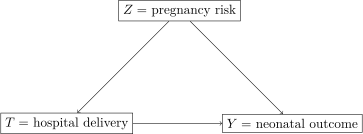
\includegraphics[width=\textwidth,height=0.4\textheight]{_tikzs/dag-delivery.png}

}

\caption{\label{fig-dag-delivery1}}

\end{figure}%

\begin{itemize}
\tightlist
\item
  assumptions:

  \begin{itemize}
  \tightlist
  \item
    women with high risk of bad neonatal outcomes
    (\texttt{pregnancy\ risk}) are referred to the hospital for delivery
  \item
    hospital deliveries lead to better outcomes for babies as more
    emergency treatments possible
  \item
    both \texttt{pregnancy\ risk} and \texttt{hospital\ delivery} cause
    \texttt{neonatal\ outcome}
  \end{itemize}
\item
  the \emph{other variable} \texttt{pregnancy\ risk} is a common cause
  of the treatment (\texttt{hospital\ delivery}) and the outcome (this
  is what's called a confounder)
\end{itemize}

\subsection{Making DAGs for our
examples:}\label{making-dags-for-our-examples-1}

\subsubsection{The hernia DAG}\label{the-hernia-dag}

\begin{figure}

\centering{

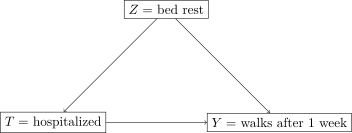
\includegraphics[width=\textwidth,height=0.4\textheight]{_tikzs/dag-hernia.png}

}

\caption{\label{fig-dag-hernia}}

\end{figure}%

\begin{itemize}
\tightlist
\item
  assumptions:

  \begin{itemize}
  \tightlist
  \item
    patients admitted to the hospital keep more \texttt{bed\ rest} than
    those who remain at home
  \item
    \texttt{bed\ rest} leads to lower recovery times thus less walking
    patients after 1 week
  \end{itemize}
\item
  the \emph{other variable} \texttt{bed\ rest} is a \emph{mediator}
  between the treatment (\texttt{hospitalized}) and the outcome
\end{itemize}

\section{DAG definitions}\label{dag-definitions}

\subsection{The DAG definition of an
intervention}\label{the-dag-definition-of-an-intervention}

assume this is our DAG for a situation:

\begin{itemize}
\tightlist
\item
  then {intervening} on variable \(T\) means removing all incoming
  arrows
\end{itemize}

\begin{figure}

\begin{minipage}{0.50\linewidth}

\centering{

\includegraphics[width=0.5\textwidth,height=\textheight]{_tikzs/dag-obs.png}

}

\subcaption{\label{fig-obs}observational data}

\end{minipage}%
%
\begin{minipage}{0.50\linewidth}

\centering{

\includegraphics[width=0.5\textwidth,height=\textheight]{_tikzs/dag-intervened.png}

}

\subcaption{\label{fig-intervened}intervened DAG}

\end{minipage}%

\end{figure}%

\begin{itemize}
\tightlist
\item
  which means \(T\) does not \emph{listen} to other variables anymore,
  but is set at a particular value, like in an experiment
\end{itemize}

\subsection{Basic DAG types}\label{basic-dag-types}

\begin{figure}

\begin{minipage}{0.33\linewidth}

\centering{

\includegraphics[width=1\textwidth,height=\textheight]{_tikzs/dag-chain.png}

}

\subcaption{\label{fig-chain}chain}

\end{minipage}%
%
\begin{minipage}{0.33\linewidth}

\centering{

\includegraphics[width=1\textwidth,height=\textheight]{_tikzs/dag-fork.png}

}

\subcaption{\label{fig-fork}fork}

\end{minipage}%
%
\begin{minipage}{0.33\linewidth}

\centering{

\includegraphics[width=1\textwidth,height=\textheight]{_tikzs/dag-collider.pdf}

}

\subcaption{\label{fig-collider}collider}

\end{minipage}%

\end{figure}%

\subsection{next steps}\label{next-steps}

\emph{conclusion 1}: seeing is not doing

\textbf{to follow-up}

\begin{itemize}
\tightlist
\item
  DAG to picture the game
\item
  doing = mutilating DAG
\item
  hotel 2: the Randtz
\item
  identifyability: more SCMs with same marginals
\item
  another hidden variable: are the guests brittish
\item
  SCM = know rules of the game
\item
  DAG = know who listens to what
\item
  why are DAGs useful? know what you can compute
\end{itemize}

\subsection{References}\label{references}




\end{document}
